\chapter{Model-View-Controller}
\section{Model View Controller}
Il \textbf{Model-View-controller} (\textbf{MVC}) è un pattern architetturale
molto diffuso nello sviluppo di sistemi software, in particolare nell'ambito
della programmazione orientata agli oggetti e in applicazioni web, in grado di
separare la logica di presentazione dei dati dalla logica di business. Partiamo
analizzando il pattern architetturale:
\begin{figure}[!ht]
      \centering
      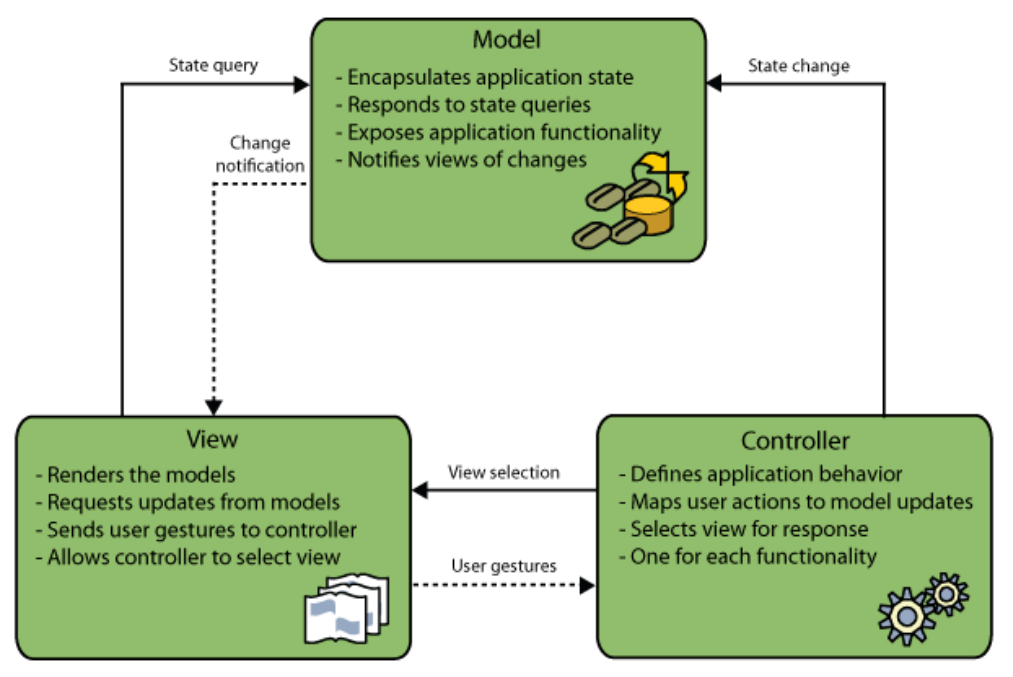
\includegraphics[width=0.5\textwidth]{img/mvc/mvcpattern.png}
      \caption{Model View Controller}
      \label{fig:enter-label}
\end{figure}

dove con le frecce piene si hanno le invocazioni di metodi e con quelle
tratteggiate gli eventi. Analizzando meglio le tre componenti si ha che:
\begin{itemize}
      \item \textbf{Model}: incapsula lo stato dell'applicazione, fornisce i
            metodi per accedere ai dati utili dell'applicazione. È implementato
            dalle classi che realizzano la logica applicativa.
      \item \textbf{View}: renderizza il modello, richiede l'aggiornamento dai
            modelli, invia le operazioni dell'utente al \textit{controller} e
            gli permette di selezionare la vista. Visualizza i dati contenuti
            nel model e si occupa dell'interazione con utenti e agenti. Presenta
            lo stato del model all'utente.
      \item \textbf{Controller}: definisce il comportamento dell'applicazione,
            riceve i comandi dell'utente (in genere attraverso la \textit{View})
            e li attua modificando lo stato degli altri due componenti. Si ha un
            controller per funzionalità. È un mediatore tra view e controller.
\end{itemize}
La \textit{view} raccoglie gli input dell'utente e li inoltra al \textit{controller},
che li mappa in operazioni sul \textit{model}, che viene modificato. A questo
punto il controller seleziona la nuova view da mostrare all'utente, che a sua
volta interagisce per avere i dati con il model. Cambi del model sono notificati
alla view per eventuali cambiamenti dei dati.

Per la costruzione del controller si hanno vari design pattern tra cui:
\begin{itemize}
      \item \textbf{Page Controller}: si ha un controller per pagina che si
            occupa di:
            \begin{itemize}
                  \item Controllare i parametri delle richieste e richiamare la
                        business logic sulla base della richiesta.
                  \item Selezionare la view successiva da mostrare.
                  \item Preparare i dati per la presentazione.
            \end{itemize}
            Si ha il seguente flusso di controllo:
            \begin{enumerate}
                  \item Il controllo si sposta dal server Web al Page Controller.
                  \item Estrae i parametri dalla richiesta.
                  \item Utilizza alcuni oggetti di business.
                  \item Decide la view successiva.
                  \item Prepara i dati da mostrare nella view successiva.
                  \item Porta il controllo (e i dati) alla view.
            \end{enumerate}
            Dal punto di vista implementativo si possono usare soluzioni con
            poca logica di controllo o con una forte logica di controllo. Con
            questo pattern si implementa un controller per ciascuna pagina
            logica, avendo, per la scalabilità, la crescita finita del controller
            proporzionale al numero di pagine necessarie, producendo un numero
            comunque finito e gestibile di file di codice piccoli.
      \item \textbf{Front Controller}: definisce un singolo componente per
            gestire tutte le richieste. Ogni volta che si riceve una richiesta,
            il front controller rappresentato dall'\textbf{handler} si avvale
            della collaborazione di una gerarchia di classi, le quali
            rappresentano i comandi che possono essere richiesti dall'utente
            attraverso l'interfaccia. Questo approccio risulta scalabile perché
            al crescere della dimensione dell'applicazione ciò che cresce non è
            l'handler ma cresce la gerarchia dei comandi. Nel dettaglio l'handler:
            \begin{itemize}
                  \item Riceve la richiesta dal server.
                  \item Esegue operazioni generali/comuni a tutti i comandi.
                  \item Decide l'operazione che deve essere eseguita e alloca
                        l'istanza del comando.
                  \item Delega l'esecuzione al comando istanziato.
            \end{itemize}
            mentre il comando:
            \begin{itemize}
                  \item Estrae i parametri dalla richiesta.
                  \item Invoca metodi implementati nella business logic.
                  \item Determina la vista successiva.
                  \item Dà il controllo al View.
            \end{itemize}
            Il front controller è più complesso del page controller. Inoltre
            evita la duplicazione del codice tra i vari controller, permette una
            semplice configurazione del server avendo una sola servlet, permette
            di gestire dinamicamente nuovi comandi, facilita l'estensione del
            controller e i comandi possono essere implementati sia come metodi,
            sia come classi. Al crescere dell'applicazione cresce la gerarchia
            di comandi, mantenendo quasi invariato il front controller.
      \item \textbf{Intercepting Filter}: è utile per gestire richieste e
            risposte prima che vengano servite. Viene spesso usato insieme al
            front controller per “decorare” richieste e risposte con funzioni
            aggiuntive.

            Dal punto di vista implementativo il web server fornisce Filter
            Manager e Filter chain, dovendo quindi implementare e dichiarare
            solo i filters.
            \begin{figure}[!ht]
                  \centering
                  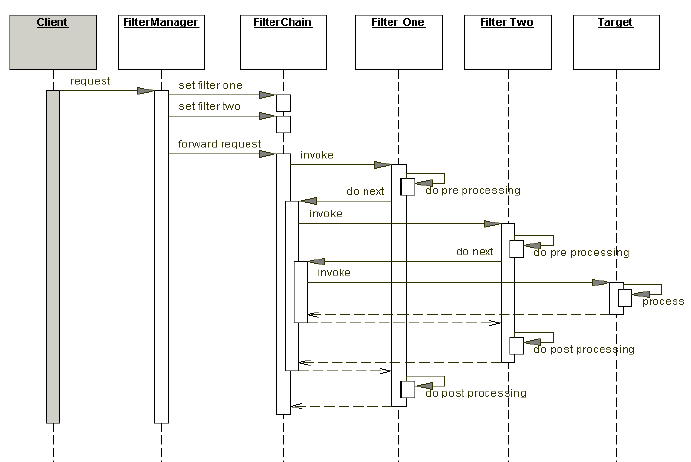
\includegraphics[width=0.5\textwidth]{img/mvc/filter.png}
                  \caption{Comportamento del Intercepting Filter}
            \end{figure}
            I filtri sono composti da:
            \begin{itemize}
                  \item \textbf{preprocessing}: operazioni prima delle invocazioni.
                  \item \textbf{invocazione}: si invocano le funzionalità della
                        filter chain.
                  \item \textbf{postprocessing}: operazioni dopo le invocazioni.
            \end{itemize}
      \item \textbf{Application Controller}: usato in quanto all'aumentare della
            complessità del flusso, la gestione del flusso potrebbe essere
            concentrata in una classe. Solitamente viene usato dal page controller
            o dal front controller.
\end{itemize}
Possiamo definire anche i design pattern per l'implementazione della \textit{view}:
\begin{itemize}
      \item \textbf{Template View}: che genera codice HTML dalle pagine template
            che includono chiamate al modello. Dove nel codice HTML si hanno vari
            marker e l'\textbf{helper} genera i dati del dominio e separa la vista
            dalla logica di implementazione.

            L'helper è creato dal controller ed è accessibile da una vista. L'helper
            fornisce l'accesso ai dati del Model nella vista, quest'ultimo passato
            dal controller. In questo modo si possono accedere ai dati utilizzando
            getter specifici.
      \item \textbf{Transformation View}: che trasforma le entità di dominio in
            HTML. Dove per il model tipicamente ogni classe implementa un metodo
            \textit{.toXML()} mentre per il transformer si ha tipicamente
            l'implementazione tramite \textit{eXtensible Style Language for
                  Transformations} (XSLT). Si ha quindi che ci si concentra
            sull'entità che deve essere trasformata, piuttosto che sulla pagina
            di output. Si ha una produzione interamente dinamica della pagina da
            parte del transformer. Il transformer legge la conversione XML e le
            regole XSLT, crea la pagina dinamicamente, inserendo i dati del model
            definito come XML nel posto specificato dalle regole XSLT.

            Purtroppo è difficile includere la logica di implementazione nella
            view anche se il testing è facile. È facile da applicare a dati in
            formato XML anche se What You See Is What You Get (WYSIWYG) sarebbe
            più intuitivo e facile da implementare. Al contrario di template view
            non vediamo cosa stiamo facendo fino a che non visualizziamo.
            Template view è usato spesso per costruire solo parti di pagine.
      \item \textbf{Two-Steps View} dove si ha la generazione della pagina HTML
            in due passaggi:
            \begin{enumerate}
                  \item Si genera un pagina logica.
                  \item Si renderizza la pagina.
            \end{enumerate}
            Spesso collassano in un'unica fase.

            Dal punto di vista implementativo si può implementare secondo due
            metodologie:
            \begin{itemize}
                  \item 2 passi XSLT: Una sequenza di due trasformazione XSLT,
                        la prima per la costruzione della pagina logica e la
                        seconda per il suo render.
                  \item template-view: Una vista template con tag custom, la
                        pagina HTML è quindi la pagina logica e i tag custom il
                        render.
            \end{itemize}
            Si ha che il “Look \& Feel” è facile da cambiare perché il rendering
            non è ottenuto tramite interazione con la strutturazione delle
            informazioni che devono essere visualizzate nella pagina.
\end{itemize}
\section{Object Relational Mapping}
Come sappiamo non si ha una relazione diretta tra programmazione a oggetti e
modello relazionale. Per questo si usa l'\textbf{Object Relational Mapping}
(\textbf{ORM}) quando si lavora con la programmazione a oggetti e dati persistenti
in un database con le classi che vanno \textit{mappate} nelle entità e viceversa.
Molti dei concetti si applicano ad altri mapping con modelli anche NoSQL. Si
sfrutta quindi un \textbf{API gateway} tra il client e le risorse dati che
“incapsula” l'accesso a una risorsa esterna con una classe e traduce le
richieste di accesso alla risorsa esterna in chiamate all'API. Con questo
approccio si nasconde l'accesso alle risorse e la complessità delle API.

Si hanno tipicamente 4 pattern per il database gateway:
\begin{itemize}
      \item \textbf{Table Data Gateway}: che prevede un oggetto per tabella.
            Prevede classi stateless ed è comodo nel paradigma procedurale ma
            meno in quello ad oggetti, in quanto i metodi ritornano dati row e
            non oggetti.
      \item \textbf{Row Data Gateway}: che prevede un oggetto per record. Si
            possono avere più copie di oggetti persistenti in memoria, avendo
            una classe gateway che funge da alter-ego del database che viene
            chiamata dalla classe coi metodi finder.
      \item \textbf{Active Record}: che prevede un oggetto per record.
      \item \textbf{Data Mapper}: che prevede un layer applicativo dedicato
            all'ORM.
\end{itemize}
\subsection{Active record}
Le classi che modellano i dati che devono essere persistenti, vengono arricchite
con metodi per permettere l'interazione col database. Un \textbf{active record}
include quindi:
\begin{itemize}
      \item La business logic.
      \item Il mapping logico al database, avendo  metodi statici come
            \textit{finder} (invocabili avendo accesso alla classe) che comunque
            restituiscono risultati già nel dominio (oggetti o collezioni di
            oggetti) e non statici i metodi gateway per lavorare con le istanze.
\end{itemize}
Tra i metodi abbiamo quindi:
\begin{itemize}
      \item \textbf{Load}: che crea un'istanza a partire dai risultati di una
            query SQL. Potrebbe essere necessario creare altri oggetti con
            accesso a più tabelle nei casi di reference.
      \item \textbf{Costruttore}: per creare nuove istanze che saranno poi rese
            persistenti invocando metodi appositi.
      \item \textbf{Finder} (statici): che incapsulano la query SQL e ritornano
            una collezione di oggetti.
      \item \textbf{Write}: tra cui si hanno:
            \begin{itemize}
                  \item \textbf{Update}: per aggiornare un record a seconda dei
                        valori degli attributi.
                  \item \textbf{Insert}: per aggiungere un record a seconda dei
                        valori degli attributi.
                  \item \textbf{Delete}: per cancellare il record corrispondente
                        all'oggetto in analisi.
            \end{itemize}
            serve sincronizzazione tra oggetto in memoria ed entità nel database.
            Per farlo si ha un attributo identificatore nella classe che compare
            anche nel record e che serve per trovare il record corrispondente ad
            un oggetto.
      \item \textbf{Getter} e \textbf{Setter}: che a seconda del caso devono
            essere subito sincronizzati con il database.
      \item \textbf{Business}.
\end{itemize}
Non è il metodo migliore dal momento che nella stessa classe ho sia i metodi
della logica di business, sia i metodi per il mapping nel database. In aggiunta,
forza anche la corrispondenza perfetta tra OOP e ER design. Il lato positivo è
la semplicità.
\subsection{Data mapper}
Con il pattern \textbf{Data Mapper} invece si ha un layer software indipendente,
dedicato alla persistenza e all'ORM, in modo che la logica di dominio non conosca
la struttura del database e nemmeno le query SQL. Si usano quindi interfacce per
consentire l'accesso ai mapper indipendentemente dalla loro implementazione.

Framework moderni implementano questo tipo di pattern (che offre la parte di
mapping senza doverli implementare, ma solo configurare).
\subsection{Ulteriori pattern ORM}
In generale si hanno dei pattern di comportamento per risolvere altri problemi
di ORM:
\begin{itemize}
      \item \textbf{Unit of work}
      \item \textbf{Identity map}
      \item \textbf{Lazy load}
\end{itemize}
e anche pattern strutturali:
\begin{itemize}
      \item \textbf{Value holder}
      \item \textbf{Identify field}
      \item \textbf{Embedded value}
      \item \textbf{LOB}
\end{itemize}
\subsubsection{Unit of work}
In questo caso si approfondiscono le operazioni ACID cercando di capire quando
sincronizzare le informazioni in memory con il database. Questo aspetto è
importante introducendo il concetto di \textbf{business transaction} per
operazioni con semantica di tipo all or nothing dove o si accettano tutte le
operazioni richieste o nessuna. Le business transaction vanno quindi mappate
nelle \textbf{system transaction} fatte dal sistema sul database.

Si hanno varie soluzioni:
\begin{itemize}
      \item \ref{fig:bt-uguale-st} aggiornare il database ogni volta che si ha
            una modifica in memoria. Si lega la business transaction con la
            system transaction. Infattibile perché si avrebbe che la transazione
            del database sarebbe troppo lunga, comportando che l'aggiornamento
            impedisce l'accesso agli altri.
            \begin{figure}[!ht]
                  \centering
                  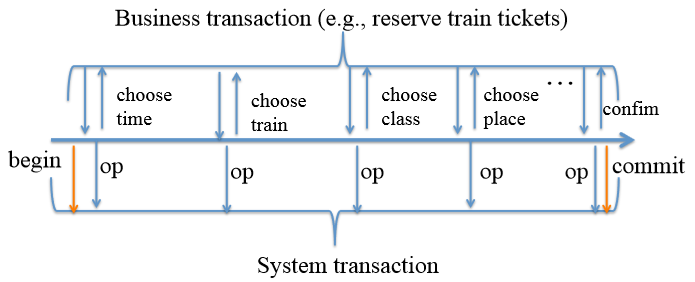
\includegraphics[width=0.5\textwidth]{img/mvc/bt-uguale-st.png}
                  \caption{System transaction uguale alla Business transaction}
                  \label{fig:bt-uguale-st}
            \end{figure}
      \item \ref{fig:op-uguale-st} aggiornare il database ad ogni modifica in
            memoria. Per la business transaction si hanno tante system transaction
            una per ogni modifica. Si rischia inconsistenza perché si hanno
            diversi aggiornamenti ma in periodi diversi.
            \begin{figure}[!ht]
                  \centering
                  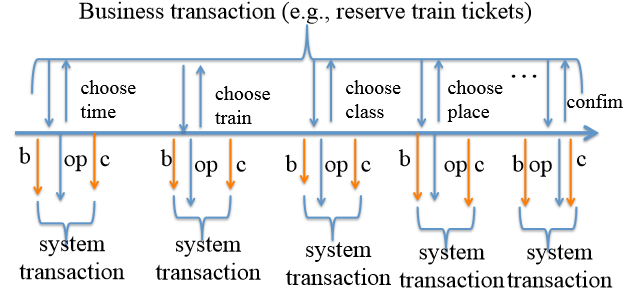
\includegraphics[width=0.5\textwidth]{img/mvc/op-uguale-st.png}
                  \caption{System transaction per ogni singola operazione nella
                        Business transaction}
                  \label{fig:op-uguale-st}
            \end{figure}
      \item \ref{fig:bt-uguale-st1} aggiornamento finale al termine della business
            transaction.
            \begin{figure}[!ht]
                  \centering
                  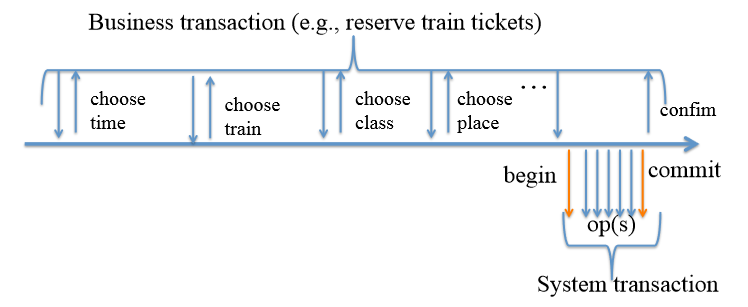
\includegraphics[width=0.5\textwidth]{img/mvc/st-finale.png}
                  \caption{System transaction alla fine della Business transaction}
                  \label{fig:bt-uguale-st1}
            \end{figure}
\end{itemize}
La \textbf{unit of work} quindi traccia ogni cambiamento (coi metodi register) e
lo attuta in una singola system transaction finale (con il commit). Per fare
questo incapsula ogni update/insert/delete, mantenendo l'integrità del database
ed evitando deadlock.

A proposito di \textit{locking} si ha che due business transaction possono essere
attive nello stesso momento e bisogna capire come devono lavorare sul database.
In questo caso si hanno due strategie:
\begin{itemize}
      \item \textbf{Optimistic locking}: usato quando si hanno poche probabilità
            di generare conflitti, avendo diversi utenti che lavorano spesso su
            dati differenti, quindi ci si basa su un numero di versione che specifica
            la versione di aggiornamento dell'oggetto.
            Due business transaction possono quindi
            interferire accedendo e modificando i record, si sfrutta il numero
            di versione per tenere traccia delle modifiche applicate sull'oggetto.
            Nel momento in cui in una business transaction stiamo per effettuare
            un'operazione di modifica, per prima cosa leggiamo il numero di versione
            dell'oggetto, se questo è uguale all'ultimo numero di versione allora
            si effettua la modifica aggiornando anche il numero di versione,
            altrimenti si cancella la business transaction e si ricarica il record.
      \item \textbf{Pessimistic locking}: usato quando hanno alte probabilità di
            generare conflitti. Gli oggetti sono bloccati non appena vengono
            usati riducendo la concorrenza. Non si permette quindi alle
            transazioni di lavorare concorretemene riducendo però le prestazioni
            del sistema ma aumentando la sicurezza.
\end{itemize}
Poi, per avvisare la unit of work che un'operazione di persistenza è stata
schedulata, si hanno due pattern:
\begin{itemize}
      \item \textbf{Caller registration}: dove chi modifica l'entità lo notifica
            direttamente alla unit of work. Questa soluzione è rischiosa in quanto
            il programmatore potrebbe dimenticarsi ma permette maggior
            flessibilità, permettendo di decidere dinamicamente se i cambiamenti
            devono “riflettersi” sullo storage persistente.
      \item \textbf{Object registration}: dove è l'entità modificata a notificare
            la unit of work, che però deve obbligatoriamente avere accesso globale.
            Ogni cambiamento viene comunque notificato. Solitamente si usa questa
            soluzione ma nella variante in cui le classi persistenti non includono
            il codice per la notifica, ma tramite una strumentazione trasparente
            offerta dai framework.
\end{itemize}
\subsubsection{Identity map}
In questo caso si studia il load di un'istanza direttamente a partire dal database.
Se un certo record viene richiesto due volte si generano due oggetti uguali.
In pratica uno stesso oggetto può essere caricato più volte, o da azioni differenti
dello stesso utente rischiando di creare inconsistenze, ad esempio se una istanza
viene modificata. Questo porta ad avere dati inconsistenti, oltre a questo può
essere presente una ridondanza di dati e in determinati casi problemi di
sicurezza in quanto utenti diversi possono cercare di forzare queste
inconsistenze in modo intenzionale.

\textbf{Identity map} è quindi un oggetto con la responsabilità di identificare
gli oggetti caricati in una sessione, funzionando come una sorta di cache,
controllando l'eventuale presenza dell'oggetto “in cache” prima di caricarne uno
nuovo dal database. Se l'oggetto è già presente si ritorna un riferimento
all'oggetto. Identity map quindi mantiene i riferimenti agli oggetti tramite un
sistema chiave-valore.

Generalmente la chiave della mappa è quella primaria del database. Si hanno
diverse identity map:
\begin{itemize}
      \item Una per applicazione, se chiavi di entità differenti sono disgiunte.
      \item Una per classe.
      \item Una per tabella, generalmente meglio se una per classe.
\end{itemize}
\subsubsection{Lazy load}
A volte è necessario avere solo una parte di un oggetto per eseguire una certa
operazione anche perché alcuni attributi possono essere particolarmente pesanti.
Si parla quindi di efficienza.

Si procede quindi con il pattern lazy load che crea oggetti inizializzando solo
alcuni attributi lasciando comunque possibilità di caricare in seguito ulteriori
attributi non ancora inizializzati se ce ne fosse necessità, in modo on-demand,
tramite i finder.
\subsubsection{Value holder}
Con questa tecnica si usa un oggetto, ossia il value holder, come uno storage
intermediario per un attributo. Anche in questo caso si ha un'inizializzazione
“lazy” implementata da questo oggetto che caso per caso potrebbe essere istanziato
con diverse strategie di load. Si separa la logica di dominio da quella “lazy”
di loading.
\subsubsection{Identify field}
Normalmente si hanno:
\begin{itemize}
      \item L'identità in memory rappresentata dalla reference dell'oggetto.
      \item L'identità nel database rappresentata dalla chiave primaria.
\end{itemize}
e si ha bisogno di accoppiare/sincronizzare le due identità per la consistenza
dei dati.

La soluzione è usare l'identity field ovvero un “nuovo” attributo nell'oggetto
il cui valore diventa la “chiave primaria” (solitamente chiamato id, di tipo long).
Non si usano i normali attributi/identificatori della classe perché potrebbero
modificare nel tempo di sviluppo del programma.

Si hanno infatti due tipi di chiave:
\begin{itemize}
      \item Una chiave derivata da attributi dell'oggetto, questo comporta
            che in caso di future modifiche, queste potrebbero impattare anche
            sulla chiave dell'oggetto, portando a inconsistenze tra oggetti e
            persistenza.
      \item Chiavi dedicate, si utilizzano chiavi dedicate, autogenerate, sepesso
            di tipo long che ben supporta il check di uguaglianza (==).
\end{itemize}
Si hanno varie strategie per la generazione delle chiavi:
\begin{itemize}
      \item Direttamente dal database (con sequenze o id delle colonne).
      \item Tramite GUID, ovvero Globally Unique IDentifier, tramite opportuni
            software e librerie.
      \item Dall'applicazione, principalmente in due modi:
            \begin{itemize}
                  \item \textbf{Table scan}: usando una query SQL per determinare
                        il valore della prossima chiave.
                  \item \textbf{Key table}: usando tabelle speciali con il nome
                        delle altre tabelle e il valore successivo della chiave.
            \end{itemize}
\end{itemize}
I moderni framework ORM supportano i vari design pattern appena discussi e quelli
mancanti, relativi a chiavi esterne, cascading, ereditarietà $\dots$ In ogni caso
i pattern appena discussi sono tutti supportati dai moderni framework ORM.
\subsubsection{Embedded value}
Con questo pattern si hanno semplici oggetti, senza un chiaro concetto di
identità, che possono essere inclusi in oggetti che fungono da alter-ego delle
tabelle anziché creare tabelle dedicate.
\subsection{JPA}
\textbf{Java Persistence API} (JPA) è uno standard di implementazione di ORM nel
linguaggio Java. Questa implementazione consiste in un grande set di pattern/
meccanismi già implementati mediante:
\begin{itemize}
      \item Sistema di annotazioni.
      \item Servizi
\end{itemize}
Si hanno 4 macro-elementi:
\begin{itemize}
      \item \textbf{Database}: che salverà degli oggetti, istanze di entity class,
            classi con un mapping ad un record. Il mapping è garantito attraverso
            le annotazioni.
      \item Classi della logica di dominio.
      \item \textbf{Entity manager}: servizio che permette di lavorare sulle entità
            persistenti
      \item gestione delle transazioni
\end{itemize}
\subsubsection{Entity manager}
Gli oggetti persistenti sono anche chiamati come \textbf{Pojo} (\textit{Plain Old
      Java Objects}) perché oggetti normali Java ma con annotazioni. Sono uguali
fino a quando non interagiscono con l'entity manager.

Ogni Pojo in memoria può trovarsi in 2 stati:
\begin{itemize}
      \item \textbf{managed}: entity manager è consapevole nella presenza in
            memoria.
      \item \textbf{unmanaged}: entity manager non è consapevole nella presenza
            in memoria.
\end{itemize}
Essenziale lo stato per implementare il pattern Unit of Work e Identity map.
In caso di creazione o cancellazione di entità dobbiamo notificarlo alla Unit of
Work mentre nel caso di modifica queste vengono applicate automaticamente.
Entity Manager cattura le notifiche in modo trasparente.

Un'entità diventa managed quando si crea da una classe con annotazione
\textit{entity}, mentre è considerata unmanaged quando viene scambiata tra diverse
parti. In questo caso bisogna notificarlo all'Entity Manager.

Il servizio Entity Manager è in grado di gestire solo le classi che dichiariamo
(insieme di classi persistenti = persistence unit) e vengono dichiarati nel file
persistence.xml e si deve specificare una connessione al database. A runtime la
persistence unit si chiama persistence context. (si possono dichiarare più
persistence unit e context)

L'annotazione @Entity specifica un oggetto persistente e avremo una tabella
per memorizzare gli oggetti con le colonne con gli stessi nomi degli attributi.
Si possono utilizzare annotazioni per modificare il mapping come i nomi dei
fields e delle tabelle.

Definito il mapping utilizzeremo Entity Manager per accedere ai dati. Creiamo
l'Entity Manager e per notificare la creazione si usa la funzione di persist.
(UoW) La scrittura non è immediata perché aspetta quando si aprirà la transazione.
Dall'Entity Manager posso recuperare l'entità con i metodi finder che chiedono la
classe dell'oggetto richiesto e id. Il risultato dei metodi sono sempre oggetti.
getReference è caricamento Lazy.
Un altro modo di estrazione degli oggetti è attraverso una query simile a SQL,
non si usano i nomi delle tabelle o field delle tabelle ma bensì si usano nomi delle
classi e attributi (sempre secondo object oriented).
Per modificare le entità si modificano gli attributi e alla prossima transazione
verrà salvata in automatico. La modifica non viene riportata al database se
l'entità è unmanaged. Per renderla effettiva allora si usa merge che:
\begin{itemize}
      \item se l'entità non esiste allora viene inserita.
      \item se esiste un'altra entità si sovrascrive l'unmanaged sul database.
\end{itemize}
Utilizzando il metodo refresh posso aggiornare i campi dell'entità con i valori
dei campi che sono salvati all'interno del database.

Per aprire e chiudere la transaction ci sono dei metodi dell'Entity Manager.

SequenceGen(nome generatore in Java, nome generatore nel database)

Cerca di usare sempre un'attributo ad hoc per le chiavi.

Possiamo fare il mapping di un'entità su più tabelle con SecondaryTable e l'entità
sarà partizionata tra le due tabelle che hanno i record associati con lo stesso
id. Utile per accedere a database legacy e codificare più tabelle in un'entità.

Mapping delle associazioni comportano il caricamento anche delle entità associate.
Vediamo ora come implementare le associazioni:
\begin{itemize}
      \item \textbf{One-to-One} mono-direzionale: si hanno due modi per mappare
            una relazione 1 a 1:
            \begin{enumerate}
                  \item Utilizzando una chiave esterna nella tabella padre che punta
                        alla tabella figlia.
                  \item Effettuando la join sulle chiavi primarie, in questo modo
                        si ha un entità suddivisa in due tabelle.
            \end{enumerate}
      \item \textbf{One-to-Many} mono-direzionale: nella parte a 1 si memorizza
            una collection della parte a molti. Questo può essere gestito con una
            tabella di join, specificando il nome della tabella e le chiavi da
            utilizzare.
      \item \textbf{Many-to-One} mono-direzionale: si applica lo stesso ragionamento
            della one-to-many invertendo i ruoli.
      \item \textbf{Relazioni bidirezionali}: sono raramente utilizzate. Si possono
            creare aggiungendo un campo in entrambe le classi e specificando in una
            delle due entità il mapping al campo della classe a cui fare riferimento.
      \item \textbf{Many-to-Many}: si crea una tabella di join utilizzando le
            chiavi primarie delle due entità. Nelle classi è possibile esprimere
            un campo di tipo collection che rappresenta gli elementi dell'altra
            classe che partecipa alla relazione.
\end{itemize}
\begin{nota}
      Utilizzando questo approccio si progettano direttamente le classi e non il
      database.
\end{nota}
Dato che nella programmazione a oggetti posso avere delle gerarchie tra gli
oggetti, ma questi non sono supportati dal modello relazionale, si ha la necessità
di mappare le gerarchie. Il mapping deve essere fatto in modo esplicito:
\begin{itemize}
      \item \textbf{Single table}: tutto in una tabella e si introduce un attributo
            discriminatore. Richiede che sia possibile avere null negli attributi.
            Veloce e semplice ma si vincola ad non avere not null.
      \item \textbf{1 tabella per classe}: dove ogni classe ha una tabella
            associata con un campo per ogni attributo. Tutti gli attributi di una
            classe sono quindi in una singola tabella dedicata. Si ha un maggior
            controllo dei vincoli e un mapping ancora semplice ma è difficile
            da gestire con l'Entity Manager e il DBMS deve supportare la SQL
            UNION.
      \item \textbf{1 tabella per sottoclasse}: dove si ha una classe per tabella
            ma senza una copia degli attributi per le classi figlie, le quali sono
            caratterizzate solo dall'id e dagli attributi extra rispetto alla
            classe padre. Si ha quindi un mapping “uno a uno”. Questa strategia
            supporta i vincoli tabellari e non richiede la SQL UNION ma si ha un
            istanza “suddivisa” su più tabelle ed è generalmente una soluzione
            lenta in esecuzione (dovendo eseguire i join).
\end{itemize}
Si mappa Ereditarietà perché permette di ridurre la duplicazione e di risolvere
le query correttamente.
\section{Gestione delle dipendenze}
Vogliamo sviluppare codice in classi che siano il più indipendenti possibili e
con più disaccoppiamento possibile, si può considerare ciascuna classe come un
singolo componente, le quali possono essere componibili tra di loro per risolvere
un problema o implementare un servizio. Mantenendo l'indipendenza tra i componenti
del sistema si introduce una semplicità nella fase di manutenzione e evoluzione
del sistema.

Le dipendenze tra i componenti possono essere soddisfatte in due modi:
\begin{itemize}
      \item \textbf{Dinamicamente}: a runtime i componenti indipendenti vengono
            collegati, quindi si ha alto disaccoppiamento.
      \item \textbf{Staticamente}: si inserisce all'interno del componente parte
            del codice del componete dipendente, in questo caso si ha una mancanza
            di disaccoppiamento perché la classe sarà meno riutilizzabile, dal
            momento che, esportandola, esporteremo anche la classe dipendente.
\end{itemize}
Nella gestione delle dipendenze un aspetto fondamentale è il \textbf{decoupling},
ovvero si rendono indipendenti le componenti da pubblicare anche se a runtime tali
componenti devono comunque interagire.

Si hanno quindi alcuni design pattern per gestire le dipendenze dinamicamente:
\begin{itemize}
      \item \textbf{Inversion control}: si ha un elemento esterno che definisce
            il valore della dipendenza, servizio che riempie i riferimenti
            dall'esterno (dependency injection).
      \item \textbf{Service locator}: si implementa un componente che gestisce
            le dipendenze per accedere ai componenti, in questo caso i riferimenti
            non vengono risolti in modo automatico, ma sarà il componente che
            manualmente farà richiesta al servizio di registry che ritornerà il
            componente cercato.
\end{itemize}
\subsection{Inversion control (Dependency Injection)}
Si utilizza un componente esterno, chiamato \textbf{assembler} che si occupa di
connettere i componenti in automatico a runtime senza una loro effettiva richiesta.

La dipendenza viene risolta, attraverso l'assembler, alla creazione dell'oggetto
in modo trasparente. Questa operazione può essere fatta tramite:
\begin{itemize}
      \item \textbf{Costruttore}: si ha un attributo della classe che rappresenta
            la dipendenza e lo si inizializza attraverso il costruttore.
      \item \textbf{Metodi setter}: si ha un attributo della classe che rappresenta
            la dipendenza e lo si inizializza attraverso uno specifico metodo
            setter.
      \item \textbf{Interfacce}: si ha un attributo della classe e un'interfaccia
            che dichiara il setter, l'assembler utilizza il metodo setter definito
            nell'interfaccia per risolvere la dipendenza. (utilizzata raramente)
      \item \textbf{Reflection}: non si utilizza un metodo ma bensì le annotazioni.
            In Java, si utilizza @Autowired la quale specifica che deve essere
            risolta la dipendenza e con @Component che specifica cosa utilizzare
            per riempire gli Autowired.
\end{itemize}
Generalmente l'assembler viene fornito dal framework e può essere configurato
utilizzando un file di configurazioni o attraverso delle annotazioni.
\begin{figure}[!ht]
      \centering
      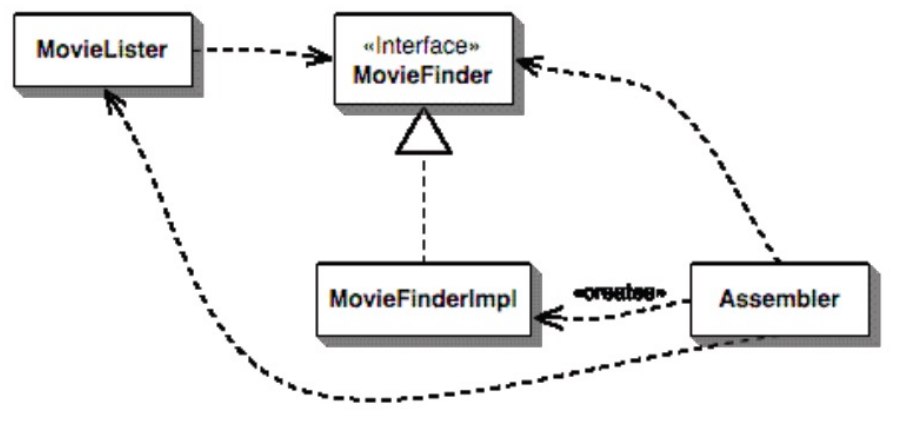
\includegraphics[width=0.5\textwidth]{img/mvc/inversion-control.png}
      \caption{Inversion control implementation}
\end{figure}
\subsection{Service locator (Dependency lookup)}
Si utilizza una classe che implementa servizio di locazione, solitamente si
realizza utilizzando una classe singleton la quale contiene una mappa chiave-valore
che tiene traccia dei componenti istanziati.

In sostanza, si definiscono i singoli componenti che implementano un'interfaccia
factory. Quando noi definiamo i servizi si definisce un attributo del tipo del
factory che verrà associato attraverso reflection.

A questo punto la classe che deve soddisfare la dipendenza fa un accesso al service
locator chiedendo che venga ritornato un riferimento al componente che deve essere
utilizzato.

Quando si chiama il componente si utilizza il factory che fa la chiamata al lookup.
\section{Transaction}
Importante sarà definire le transazioni quando si accede al database, questo può
essere fatto attraverso le dichiarazioni specificate con le annotazioni.

Il ciclo di vita delle transazioni è il seguente:
\begin{itemize}
      \item \textbf{inizio}: iniziano con la chiamata di un metodo che ha un'annotazione
            di apertura della transazione.
      \item \textbf{fine}: finiscono con la chiamata di un metodo che ha un'annotazione
            di chiusura della transazione.
\end{itemize}
In questo modo si separa la logica transazionale dalla logica di business perché
la prima viene gestita dal framework attraverso le annotazioni. Le annotazioni
transazionali si possono applicare alla classe (i metodi e attributi ereditano
l'annotazione) oppure a livello di metodo e attributo della classe. Se si specifica
l'annotazione a livello di classe, allora le annotazioni a livello di metodo
saranno un override di quella della classe.

Esistono vari tipi di annotazioni:
\begin{itemize}
      \item \textbf{Not supported}: il codice eseguito non fa parte della
            transazione.
      \item \textbf{Supports}: dipende dal chiamante, se c'è una transazione in
            corso anche il codice del metodo comparirà nella transazione,
            altrimenti, se non c'è la transazione allora il codice non appartiene
            alla transazione.
      \item \textbf{Required}: richiede che deve essere presente una transaction,
            se il chiamante non è in una transazione allora si avvia una nuova
            transazione, al contrario usa quella del chiamante.
      \item \textbf{RequiresNew}: crea una nuova transaction ad hoc per l'esecuzione.
      \item \textbf{Mandatory}: il codice deve essere eseguito in una transaction
            del chiamante, se il chiamante non ha attivato una transaction allora
            viene generata un'eccezione.
      \item \textbf{Never}: non deve mai essere eseguito il codice in una transazione,
            se il chiamante ha attivato una transazione allora questo ritorna
            un'eccezione.
\end{itemize}
Parlando di persistenza e transazioni parliamo anche di isolation e database
locking, ovvero quando si creano transazioni non necessariamente sono perfettamente
“isolate”. L'isolation può essere configurato per permettere un certo livello di
interferenza con la creazione temporanea di oggetti da parte di transazioni non
ancora concluse ma che possono essere letti da altre transaction. Se si modella
erroneamente la semantica transazionale allora si può avere:
\begin{itemize}
      \item \textbf{Dirty reads}: vengono letti i dati modificati da una transaction
            non ancora terminata, quindi si possono leggere dati che potrebbero
            non essere scritti sul database.
      \item \textbf{Unrepeatible reads}: transazioni che leggono lo stesso valore
            nella stessa transazione possono ritornare valori diversi. Questo
            può essere dovuto dal fatto che una transazione legge la stessa cosa
            ma tra le due letture c'è una \textit{modifica} del valore.
      \item \textbf{Phantom reads}: transazioni effettuano due letture, la seconda
            legge nuovi record che vengono \textit{inseriti} da una transazione
            tra le due.
\end{itemize}
Questo può essere risolto a livello di DBMS specificando le seguenti tipologie
di isolamento:
\begin{itemize}
      \item \textbf{Read uncommitted}: si hanno dirty reads, unrepeatible reads e
            phantom reads.
      \item \textbf{Read committed}: si hanno unrepeatible reads e phantom reads.
      \item \textbf{Repeatable read}: si ha phantom reads.
      \item \textbf{Serializable}: isolation perfetta.
\end{itemize}
Si può definire l'isolation a livello di codice con annotazioni. La scelta del
livello di isolation comporta:
\begin{itemize}
      \item \textbf{Forte indipendenza}: performance basse perché si perde
            concorrenza
      \item \textbf{Bassa indipendenza}: performance alte perché si ha
            concorrenza.
\end{itemize}